\usetikzlibrary{arrows, positioning}
\section{Grafer 2}
\subsection{Grafterminologi}

Der findes begreber til at beskrive kanter og knuder i ikke-orienterede grafer, som bl.a. beskriver hvordan knuder og kanter er orienterede i forhold til hinanden samt hvor mange knuder eller kanter, der er forbundet til en given knude.

\begin{defn}
To knuder $u$ og $v$ siges at være naboer i en ikke-orienteret graf $G$, hvis $u$ og $v$ er endepunkter i en kant $e$, og $e$ er incident med både $u$ og $v$.
\end{defn}

\begin{defn}
En mængde af alle naboer til en knude $v$ i en graf $G=(V,E)$ betegnes $N(v)$ og kaldes et nabolag af $v$. Hvis $A$ $\subseteq$ $V$, betegner $N(A)$ mængden af alle knuder i $G$, som er nabo til mindst én knude i $A$.
\end{defn}

\begin{defn}
Graden af en knude $v$ i en ikke-orienteret graf betegnes $deg(v)$ og er antallet af kanter incidente med den givne knude.  En løkke vil bidrage med to til graden af knuden. 
\end{defn}

\noindent En knude med grad 0 betegnes som værende \textit{isoleret} og har ingen incidente kanter. En knude med grad 1 betegnes som et \textit{vedhæng} og har netop én incident kant.

\begin{exmp}
Betragt grafen i Figur \ref{eksempel_nabo}. Graden af knuderne og nabolagene for knuderne kan bestemmes. Samtidig kan isolerede knuder eller vedhæng identificeres.\\
Graden af en knude i grafen i Figur \ref{eksempel_nabo} bestemmes ved at identificere antal incidente kanter til knuden. Derfor er $\textrm{deg}(A)=1$, $\textrm{deg}(B)=3$, $\textrm{deg}(C)=3$, $\textrm{deg}(D)=4$, $\textrm{deg}(E)=3$ og $\textrm{deg}(F)=2$. 
Nabolagene for de enkelte knuder er mængden af naboknuder. 
Derfor er $N(A)=\lbrace B \rbrace$, $N(B)=\lbrace A, C, D \rbrace$, $N(C)=\lbrace B, D, E \rbrace$, $N(D)=\lbrace B, C, E, F \rbrace$, $N(E)=\lbrace C, D, F \rbrace$ og $N(F)=\lbrace D, E \rbrace$. 
I grafen er A et vedhæng, og der forefindes ingen isolerede knuder.
\end{exmp}

\begin{figure}[h]
\centering
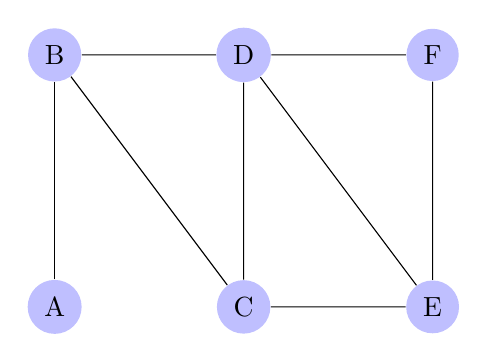
\begin{tikzpicture}
[scale=.8,auto=left,every node/.style={circle,fill=blue!25}]
  \node (n6) at (3,2) {A};
  \node (n4) at (3,6) {B};
  \node (n5) at (6,2) {C};
  \node (n1) at (6,6) {D};
  \node (n2) at (9,2) {E};
  \node (n3) at (9,6) {F};
  \foreach \from/\to in {n6/n4,n4/n5,n5/n1,n1/n2,n2/n5,n2/n3,n3/n1,n1/n4}
    \draw (\from) -- (\to);
\end{tikzpicture}
\caption{Simpel ikke-orienteret graf} \label{eksempel_nabo}
\end{figure}

\noindent For at beskrive summen af graderne for alle knuder i en graf anvendes \textit{The Handshaking Theorem}. 

\begin{thm}\label{handshake}
\textbf{The Handshaking Theorem}. Lad $G=(V,E)$ være en ikke-orienteret graf med $m$ kanter. Så er summen af knudernes grader \\
\begin{align*}
2m=\sum_{v \in V}\deg(v)
\end{align*}
\end{thm}

\begin{proof}
I en ikke-orienteret graf med $m$ kanter, bidrager hver kant i en graf med to grader - én grad til hvert endepunkt. Det samlede antal grader for alle knuder i en graf stiger således med to pr. kant og summen af $\deg(v)$ er $2m$. 
\end{proof}

\noindent Som følge af Sætning \ref{handshake} er summen af knudernes grader et lige tal. Derfor har en ikke-orienteret graf et lige antal knuder, hvor graden er et ulige tal.

\begin{thm}
En ikke-orienteret graf har et lige antal knuder af ulige grad. 
\end{thm}

\begin{proof}
Lad $V_1$ og $V_2$ være henholdsvis mængden af knuder af lige grad og mængden af knuder af ulige grad i en ikke-orienteret graf $G=(V,E)$ med $m$ kanter. Så er \\
\begin{align*}
2m=\sum_{v \in V}\deg(v)=\sum_{v \in V_1}\deg(v)+ \sum_{v \in V_2}\deg(v)
\end{align*}
Da $\deg(v)$ er lige for $v \in V_1$, er summen $\sum_{v \in V_1}\deg(v)$ også lige. Summen af de to led på højresiden i ligningen er lige, fordi de tilsammen er lig $2m$, hvorfor $\sum_{v \in V_2}\deg(v)$ også er lige. Summen $\sum_{v \in V_2}\deg(v)$ består af en række ulige tal, og for at summen bliver lige, skal der således være et lige antal ulige led i summen.
Idet summen af graderne for knuderne af ulige grad i grafen er lige, må der være et lige antal af sådanne knuder.
\end{proof}




\subsection{Repræsentation af grafer}

Der er flere brugbare måder at repræsentere grafer på, og man ønsker i hvert tilfælde at vælge den pæneste repræsentation. 
En overskuelig måde at repræsentere en graf på er ved matricer. To matricer, der almindeligvis bruges, er nabo-matricer, der er baseret på nabo-knuder, og incidens-matricer baseret på incidensen af knuder og kanter. 
Antag at $G=(V,E)$ er en simpel graf med $n$ knuder, hvor knuderne i $G$ står skrevet i vilkårlig rækkefølge som $v_1$, $v_2$, \dots , $v_n$. Nabo-matricen $A$  af G er en $n \times n$ matrix, med 1 som den $(i,j)$’te indgang når $v_i$ og $v_j$ er naboer, og 0 er den $(i,j)$’te indgang, når de ikke er naboer. Hvis nabo-matricen er $A=[a_{ij}]$ så er

\begin{align*}
a_{ij}= \left\{\begin{array}{cc}
1 & \textrm{hvis} \  \lbrace v_i, v_j \rbrace \  \in E \\
0 & \textrm{ellers} .\\
\end{array}\right.
.
\end{align*}

\noindent En nabo-matrix af en graf er baseret på den valgte ordning af knuderne, hvorfor der kan være $n!$ forskellige nabo-matricer for en graf med $n$ knuder, idet der er $n!$ forskellige måder at ordne de $n$ knuder. Nabo-matricen for en simpel ikke-orienteret graf er symmetrisk dvs. $a_{ij}=a_{ji}$, da begge indgange er 1, når de relaterede knuder er naboer, og 0 hvis de ikke er. Da en simpel graf ikke indeholder løkker, er hver indgang $a_{ii}=0$ for alle $i=1,2,3, \dots ,n$. 

Nabo-matricer kan også bruges til at repræsentere ikke-orienterede grafer med loops og flere kanter til samme knuder. Et loop ved en knude $v_i$ er repræsenteret ved 1 ved position $(i,i)$ i nabo-matricen. Når flere kanter forbinder det samme par af knuder $v_i$ og $v_j$, eller der er flere løkker ved samme knude til stede, er nabo-matricen ikke længere en nul-et matrix, idet den $(i,j)$’te indgang af matricen er lig antallet af kanter forbundet til $\lbrace v_i,v_j \rbrace$. Alle ikke-orienterede grafer, herunder multi- og pseudografer, har symmetriske nabo-matricer. \\

\noindent En anden almindelig måde at repræsentere grafer på er ved incidens-matricer. Lad $G=(V,E)$ være en ikke-orienteret graf med knuderne $v_1$, $v_2$, \dots , $v_n$ og kanterne $e_1$, $e_2$, \dots , $e_m$. Incidens-matricen, i forhold til ordningen af $V$ og $E$, er en $n x m$ matrix $M=[m_{ij}]$, hvor 
\begin{align*}
m_{ij}= \left\{\begin{array}{cc}
1 & \textrm{hvis} \  {e_j} \  \textrm{er} \  \textrm{incident} \ \textrm{med} \ v_i \\
0 & \textrm{ellers}. \\
\end{array}\right.
\end{align*}

\noindent Incidensmatricer kan også bruges til at repræsentere flere kanter og løkker. Flere kanter mellem samme to knuder er repræsenteret i incidens-matricen ved søjler med identiske indgange, idet disse kanter er incidente med det samme knudepar. Løkker er repræsenteret ved en søjle med præcis én indgang lig 1, der svarer til den knude, der er incident med løkken.

\begin{exmp}
For at illustrere eksempler på at opskrive en nabo-matrice og en incidens-matrice, betragtes grafen i Figur \ref{fig:f1}. 
\end{exmp} 

\begin{figure}[!h]
  \centering
  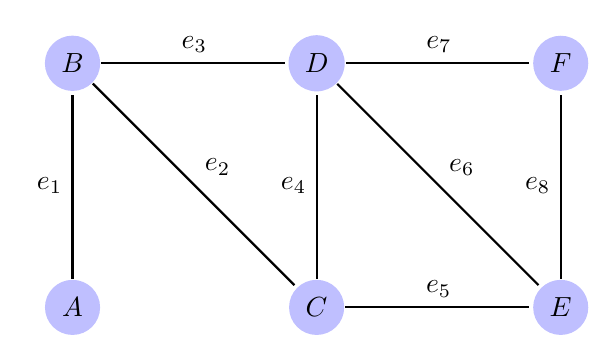
\begin{tikzpicture}
  [shorten >=1pt,node distance=3.1cm,on grid,auto]
    \tikzstyle{state}=[shape=circle,fill=blue!25,thick,minimum size=0.7cm]

    \node[state] (A) {$A$};
    \node[state,above of=A] (B) {$B$};
    \node[state,right of=A] (C) {$C$};
    \node[state,right of=B] (D) {$D$};
    \node[state,right of=C] (E) {$E$};
    \node[state,right of=D] (F) {$F$};

    \path[-,draw,thick]
    (A) edge node {$e_1$} (B)
    (B) edge node {$e_2$} (C)
    (B) edge node {$e_3$} (D)
    (C) edge node {$e_4$} (D)
    (C) edge node {$e_5$} (E)
    (D) edge node {$e_6$} (E)
    (D) edge node {$e_7$} (F)
    (E) edge node {$e_8$} (F)
    ;
  \end{tikzpicture}
  \caption{Simpel ikke-orienteret graf.}
  \label{fig:f1}
\end{figure}

\noindent Nabo-matricen $A$ for grafen i Figur \ref{fig:f1} er en $6$x$6$-matrice. Indgangen $a_{AA}=0$ angiver, at der ikke er er nogen løkker i $A$. Indgangen $a_{AB}=1$ angiver, at en kant forbinder $A$ og $B$, så $A$ og $B$ er naboer. På samme vis udfyldes resten af nabo-matricen. 

 \begin{equation*}
  \mathbf{A}=
  \begin{blockarray}{*{6}{c} l}
    \begin{block}{*{6}{>{$\footnotesize}c<{$}} l}
      A & B & C & D & E & F \\
    \end{block}
    \begin{block}{[*{6}{c}]>{$\footnotesize}l<{$}}
      0 & 1 & 0 & 0 & 0 & 0 \bigstrut[t]& A \\
      1 & 0 & 1 & 1 & 0 & 0 \bigstrut[t]&B \\
      0 & 1 & 0 & 1 & 1 & 0 \bigstrut[t]&C \\
      0 & 1 & 1 & 0 & 1 & 1 \bigstrut[t]& D \\
      0 & 0 & 1 & 1 & 0 & 1 \bigstrut[t]& E \\
      0 & 0 & 0 & 1 & 1 & 0 \bigstrut[t]& F \\
    \end{block}
  \end{blockarray}
\end{equation*} 

\noindent Incident-matricen $M$ for grafen i Figur \ref{fig:f1} er en $6$x$8$-matrice. Indgangen $m_{A,e_1}=1$ angiver, at $e_1$ er incident med $A$. Indgangen $m_{A,e_2}=0$ angiver, at $e_2$ ikke er incident med $A$ osv.

 \begin{equation*}
  \mathbf{M}=
  \begin{blockarray}{*{8}{c} l}
    \begin{block}{*{8}{>{$\footnotesize}c<{$}} l}
      $e_1$ & $e_2$ & $e_3$ & $e_4$ & $e_5$ & $e_6$ & $e_7$ & $e_8$ \\
    \end{block}
    \begin{block}{[*{8}{c}]>{$\footnotesize}l<{$}}
      1 & 0 & 0 & 0 & 0 & 0 & 0 & 0 \bigstrut[t]& A \\
      1 & 1 & 1 & 0 & 0 & 0 & 0 & 0 \bigstrut[t]&B \\
      0 & 1 & 0 & 1 & 1 & 0 & 0 & 0 \bigstrut[t]&C \\
     0 & 0 & 1 & 1 & 0 & 1 & 1 & 0 \bigstrut[t]& D \\
      0 & 0 & 0 & 0 & 1 & 1 & 0 & 1 \bigstrut[t]& E \\
     0 & 0 & 0 & 0 & 0 & 0 & 1 & 1 \bigstrut[t]& F \\
    \end{block}
  \end{blockarray}
\end{equation*}


